\section{Coarsening for Elastostatics}
In this study, we introduce data-driven finite elements (DDFEM) to 
improve the simulation speed at the cost of small inaccuracy for elastostatic problems with heterogeneous non-linear materials. DDFEM focuses on finite elements defined one a regular grid.
To handle irregular boundary geometry, we will apply the use embedded finite elements for partially filled elements.
Using regular elements enables trivial combination of fine elements into coarser blocks of elements. This operation can be applied hierarchically to coarsen a mesh multiple times.
DDFEM computation is divided into two main stages of computation---offline metamaterial construction and online coarsening.
In the offline stage, combinations of fine materials are sampled to create a database of
coarse material models. In the online stage, fine elements in a simulation model are merged and assigned appropriate coarse material model from the database.
This section will motivate algorithm design choices we made and outline the steps of DDFEM.

\paragraph{Material palettes and assignments}
This study focuses on designs made of a discrete set of materials. The methodology can be extended to handle continuous mixtures of materials.
We note that designers often do not work in a continuous space of materials but limit themselves to a relatively compact set (e.g. rubber, wood, steel) related to their problem domain. We call these discrete sets of materials palettes denoted as $\set{P}$. In this work we further limit ourselves to nonlinear hyper-elastic materials, which means that each material can be represented by a strain energy density function $V$. The palette $\set{P}$ contains a list of energy functions $\{V^1,...,V^N\}$ where $N$ is the number of distinct materials.
A material assignment to a finite element model with $K$ elements is a list of integers $(m^1,m^2,...,m^K), 1\leq m^k\leq N,$.
We also include a void (or empty) material in every palette. This allows us to perform topology changes in the same manner in which we perform material assignment updates.
In subsequent sections, we use a subscript to indicate the level of coarsening. For example, $m_0^k$ denotes the material assigned to the $k$th element at the fine scale while $m_1^k$ denotes the coarse metamaterial assigned to the finite element model resulted from the first coarsening step.

\paragraph{Conforming vs.~embedded finite elements}
The defining feature of conforming finite element methods is that the simulation mesh is aligned with the geometry of the object being simulated. One obvious feature of conforming meshes is that the mesh itself is a function of the input geometry. This means that the output of a local coarsening operator (the coarsened mesh) will also be a function of the input geometry. Also, the new material computed by each local coarsening operator will be a function of input geometry. This dependence on input geometry is a significant issue to overcome since we wish to precompute coarsened materials applicable to varying geometry in design problems. If the precomputed coarse materials depends on the material assignment and the input geometry the space of possible combinations is prohibitively large.
To mitigate this we turn to embedded finite elements. These methods embed the geometry to be simulated into the simulation mesh with no regard for whether the mesh conforms to the geometry or not. Thus an identical simulation mesh can be used for any input geometry. Local coarsening operations on the embedded mesh yield identical coarse elements and the optimized coarse material depends only on the local material distribution on the simulation mesh.  This significantly reduces the size of the coarsened material space. In this study we embed all simulation geometry into simulation meshes made of cube elements.

\paragraph{Coarsening cube elements}
\begin{figure}[ht]
	\centering	
	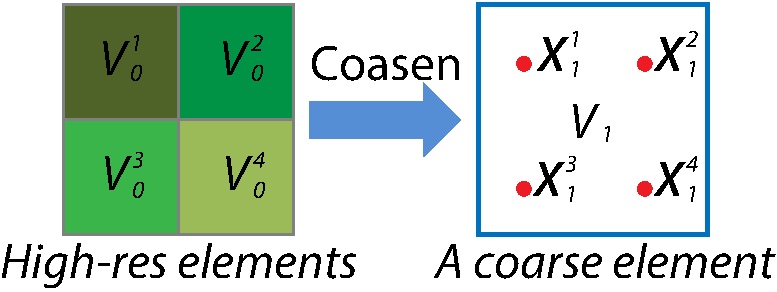
\includegraphics[width=0.5\textwidth]{images/coarsen.pdf}
	\caption{Coarsening a 2x2 block of high-resolution elements into a single coarse element.
		At each quadrature point $X_1^k$, the coarse element copies the energy density function $V_0^k$ with newly fitted material parameters to construct the coarse energy function
		$V_1$.}
	\label{fig:coarsen}
\end{figure}
The key component of our DDFEM is coarsening (Figure~\ref{fig:coarsen}). It reduces the number of elements in a finite element simulation mesh in order to improve runtime performance. Since simply removing elements can greatly reduce the accuracy of the simulation, coarsening schemes compute new material models to minimize this effect.
We regard the global coarsening of a simulation mesh as the result of many local coarsening operations which map from contiguous subsets of fine elements to coarse elements with new materials.
A local coarsening operation merges a 2x2 (2x2x2 in 3D) block of elements into a single coarse element (Figure~\ref{fig:coarsen}).
The high-resolution material assignment $(m_0^1,m_0^2,m_0^3,m_0^4)$ is mapped to a coarse metamaterial index $m_1$. We use the lookup function $L:\mathbb{N}^4\rightarrow \mathbb{N}$ to map from a list of fine material indices to a coarse material. In the actual implementation, we store $L^{-1}$, which is simply the list of fine materials that constitute each coarse material.

\paragraph{Algorithms}
With basic coarsening operation in hand, we can now define our algorithm, which is divided into two distinct phases: an \textbf{offline database construction} stage and an \textbf{online coarsening} stage.
Below we detail the input, output and steps of each stage.

\noindent\hrulefill
%\begin{algorithm}
%	\caption{Offline Database Construction}\label{alg:offline}

	\begin{algorithmic}[1]
		\Procedure{DatabaseConstruction}{ }
		\State INPUT $\set{P}_0$: Input material palette
		\State OUTPUT $\set{P}_1$: new palatte of metamaterials
		\State OUTPUT $L_0$: lookup function
        \Do
		\State Sample a new material combination $\mathbf{m}_i=(m_0^1,m_0^2,m_0^3,m_0^4)$
		\State Sample strain energy values of $\mathbf{m}_i$ under load
		\State Fit coarse material model $V_1^i$ to the sample values
		\State Add $V_1^i$ to $\set{P}_1$
		\State Store $L_0^{-1}(i) = (m_0^1,m_0^2,m_0^3,m_0^4)$
		\doWhile within computation budget
		\EndProcedure
	\end{algorithmic}
%\end{algorithm}
\hrulefill
%\begin{algorithm}
%	\caption{Online Coarsening}\label{alg:online}
	\begin{algorithmic}[1]
		\Procedure{Coarsen}{ }
		\State INPUT $\set{E}_0$: High resolution mesh with $K$ cube elements
		\State INPUT $\set{E}_1$: Coarse mesh with $L$ elements		
		\State INPUT $\{m_0^k\}$ : Material assignment
		\State OUTPUT $\{m_1^l\}$: Coarse material indices
		\ForAll{2x2 groups of $\set{E}_0$}
		  \State List high-resolution materials in the group 
		  \State $\mathbf{m}_0^k = (m_0^{k_1},m_0^{k_2},m_0^{k_3},m_0^{k_4})$
		  \State Assign coarse material $m_1^l = L(\mathbf{m}_k)$ in $\set{E}^1$
		\EndFor
		\EndProcedure
	\end{algorithmic}
%\end{algorithm}
\hrulefill

\paragraph{Hierarchical coarsening}
We stress that both stages of the DDFEM algorithm can be applied hierarchically. Given the first level of metamaterials, $\set{P}_1$, we can construct a metamaterial library, $\set{P}_2$, for the second level by using $\set{P}_1$ as an input material palette. At runtime, the coarsening algorithm looks up materials from $\set{P}_2$ to replace each 2$\times$2$\times$2 coarse block with a single element.
